\documentclass[tikz,border=6pt]{standalone}
\usepackage{xcolor}
\usetikzlibrary{arrows.meta}

\definecolor{axisgray}{HTML}{333333}
\definecolor{lineblue}{HTML}{4A90D9}
\definecolor{linered}{HTML}{E74C3C}

\begin{document}
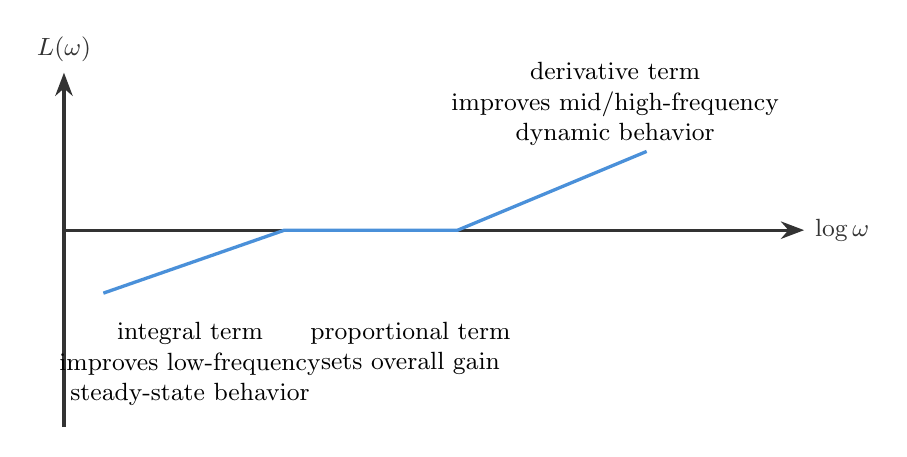
\begin{tikzpicture}[>=Stealth, line width=1.2pt, font=\small]
  \draw[axisgray, ->] (0,0) -- (9.4,0) node[right] {$\log \omega$};
  \draw[axisgray, ->] (0,-2.5) -- (0,2.0) node[above] {$L(\omega)$};
  \draw[lineblue] (0.5,-0.8) -- (2.8,0.0) -- (5.0,0.0) -- (7.4,1.0);
  \node[align=center] at (1.6,-1.7) {integral term\\improves low-frequency\\steady-state behavior};
  \node[align=center] at (7.0,1.6) {derivative term\\improves mid/high-frequency\\dynamic behavior};
  \node[align=center] at (4.4,-1.5) {proportional term\\sets overall gain};
\end{tikzpicture}
\end{document}
